\documentclass[11pt]{article}
\usepackage[margin=1.1in]{geometry}
\usepackage{amsmath,amssymb,booktabs,graphicx,natbib,hyperref,float}
\hypersetup{colorlinks=true,linkcolor=blue,citecolor=blue,urlcolor=blue}
\title{Predicting US Drug Shortages Under Trade-Policy Stress:\\
A Multi-Margin Evaluation of Tariff Exposure}
\author{Anubhaw Goyal\\ \small Independent Researcher \quad goyal.anubhaw@gmail.com}
\date{June 2026 \;--\; draft v0.2}

\begin{document}
\maketitle

\begin{abstract}
US drug shortages remain elevated while trade policy has placed unprecedented tariffs on pharmaceutical supply chains, prompting widespread concern that tariff exposure will worsen shortages. We assemble a reproducible public-data panel---4{,}017 ingredient--dosage-form units over 102 months (2018--2026)---combining FDA shortage records (with historical spells reconstructed from 44 Internet Archive snapshots of the FDA database), Orange Book market structure, NADAC acquisition prices, and trade exposure mapped from US Census import data at HS-4 level. We evaluate tariff/trade exposure on three margins. \emph{Prediction}: classifiers predict shortage onset within six months at ROC-AUC 0.785 under rolling-origin temporal validation, but trade features add no discriminative power ($\Delta$AUC $+0.001$, DeLong $p=0.88$) and, after isotonic recalibration (ECE $\le 0.001$), no proper-scoring gain. \emph{Duration}: shortage spells are long (median 28.8 months); trade \emph{structure} matters where trade \emph{flows} do not---origin-concentrated API classes resolve slowest (hormones HR 0.40, $p=0.08$) and injectables persist longer (logrank $p=0.046$). \emph{Quasi-causal}: difference-in-differences around the February 2025 IEEPA China tariffs finds no detectable differential onset ($p=0.53$) or resolution ($p=0.50$) effect through June 2026. We conclude that tariffs have not (yet) moved US drug shortages at detectable magnitudes---but origin concentration robustly predicts which shortages persist. Power limits are documented transparently: new onsets fell to historic lows in 2024--25, the enacted tariff dose on generics was modest (10--20\%), and Section~232 pharmaceutical tariffs exempt generics. All data and code are public.
\end{abstract}

\section{Introduction}
Drug shortages are a persistent failure mode of the US pharmaceutical market: between 2018 and 2023, 258 active ingredients spanning 1{,}961 drug products went into national shortage, concentrated in low-price generic sterile injectables \citep{aspe2025}. Since 2025, trade policy has become a candidate stressor: IEEPA tariffs on China (10\% from February 2025, 20\% from March, reduced to 10\% in November) reach API and generic supply chains, and Section~232 pharmaceutical tariffs (proclaimed April 2026) impose tiered rates of 0--100\% on patented products while exempting generics ``at this time'' \citep{whitehouse2026}. With roughly 72\% of API manufacturing facilities supplying the US located overseas as of 2019 \citep{woodcock2019}, the question asked by policymakers, hospital systems, and the press is direct: will tariffs cause or prolong shortages?

This paper answers with a multi-margin evaluation on public data. Our contributions: (i) the first US shortage-prediction study on FDA-era data with survival and machine-learning methods under strictly temporal validation; (ii) a novel public reconstruction of historical shortage spells from Internet Archive snapshots of the FDA database, with exact onsets and interval-censored resolutions; (iii) a three-margin evaluation of trade exposure---prediction, duration, quasi-causal---returning a carefully documented null on tariff flows alongside a robust positive on origin concentration; (iv) full reproducibility.

\section{Related work}
\citet{pall2023} predict shortages one month ahead from sales data of 22 Canadian pharmacies ($\sim$69\% accuracy), using proprietary signals without trade features or US scope. \citet{roe2025} build ML models of shortage duration and causes on South Korean regulatory data. \citet{shortagesim2025} simulate shortage dynamics under information asymmetry. \citet{aspe2025} provide the descriptive baseline for US shortages 2018--2023. None predicts US shortages from public data with survival framing, none evaluates trade or tariff exposure, and none validates across the 2024--26 regime change. % TODO v0.3: expand (Conti & Berndt economics of generic exit; tariff pass-through; interval-censored survival; clustered forecast evaluation)

\section{Data}
\paragraph{Outcome reconstruction.} The live FDA Drug Shortage Database is a snapshot: of 1{,}671 current records, only 29 are marked Resolved. We reconstruct shortage history from 44 Wayback Machine captures of the FDA CSV export (2019--2026, approximately monthly; 2022 has a single capture). A unit is in shortage at capture $t$ if any of its records is ``Current''; onsets are exact (Initial Posting Date); resolution dates are interval-censored between consecutive captures (median interval width 101 days). Our reconstructed onset counts track FDA's reported 15 new shortages in CY2024 \citep{fda2024counts} and ASHP's 89 new shortages in 2025, a twenty-year low \citep{ashp2025}.

\paragraph{Unit of analysis and entity resolution.} Units are ingredient $\times$ dosage-form buckets: 4{,}017 marketed units, 372 spells, 320 onsets from 2018. Ingredient matching to the Orange Book and NDC directory uses three tiers (exact; salt/hydrate-stripped; component-wise for combinations), covering 94.7\% and 98.7\% of shortage records respectively; residuals are identified (biologics, parenteral-nutrition components). Company-level units were rejected because only 35\% of FDA shortage companies match NDC labelers by name.

\paragraph{Features.} Domestic block: manufacturer counts, generic (ANDA) share, dosage form, ingredient age, NADAC price level and 12-month change (11.7M weekly observations), and trailing shortage history (leakage-free). Trade block: HS-4 API-heading origin mix from Census import data---China and India import shares, origin Herfindahl, import growth---plus verified policy timelines (IEEPA rates; \S232 anticipation and enactment) and a China-tariff-exposure interaction. Aggregate rows (EU, NATO) in the Census extracts were identified and removed; corrected origin shares match known patterns (China 38\% of vitamin imports, 26\% of antibiotics; India 40\% of other organic APIs).

\section{Methods}
Evaluation is rolling-origin temporal only: four folds (test years 2021, 2022, 2023, 2024--25), predictions pooled (n = 223{,}740 unit-months; 79 events). Feature-set comparisons are paired on identical rows: DeLong tests on AUC \citep{delong1988}; Diebold--Mariano tests on Brier loss \citep{diebold1995}, both naive and clustered by unit. Probabilities are recalibrated with isotonic regression fit on early folds and applied to the 2024--25 fold; decision relevance uses decision-curve analysis \citep{vickers2006}. Duration uses Kaplan--Meier with interval-censoring sensitivity (lower/mid/upper conventions), Cox proportional hazards with Schoenfeld diagnostics, and a random survival forest comparison. The quasi-causal margin is a difference-in-differences design: treatment = top tercile of China import share (fixed at January 2025), post = February 2025 (IEEPA), unit-clustered standard errors; outcomes are next-month onset (on the not-in-shortage risk set) and next-month resolution (on the in-shortage set).

\section{Results}
\subsection{Onset prediction}
Logistic regression attains pooled out-of-sample ROC-AUC 0.785 (stable across folds); LightGBM does not improve on it at 79 pooled events. Standardized coefficients (Figure~\ref{fig:coef}) are led by injectable form ($+1.42$), ingredient age ($+1.03$), and falling prices (12-month price change $-0.28$): price \emph{declines} predict onset, consistent with deflation-driven supplier exit. At the three-month horizon the picture is unchanged (ROC 0.756).

\begin{table}[H]\centering\small
\caption{Trade ablation (H3): paired comparison on identical rows, pooled out-of-sample 2021--25 (n = 223{,}740; 79 events).}
\begin{tabular}{lcccc}
\toprule
 & AUC & $\Delta$AUC & DeLong $p$ & Brier (recalibrated) \\
\midrule
Logistic, domestic & 0.7847 & --- & --- & $9.903\times10^{-5}$ \\
Logistic, + trade  & 0.7856 & $+0.0010$ & 0.877 & $9.899\times10^{-5}$ \\
\bottomrule
\end{tabular}
\label{tab:ablation}
\end{table}

\subsection{Trade ablation}
Table~\ref{tab:ablation}: trade features add no discrimination ($\Delta$AUC $+0.001$, $p=0.88$). The raw-probability Brier improvement survives unit-clustered DM testing ($p=1.4\times10^{-10}$) but vanishes after isotonic recalibration ($\Delta \approx 4\times10^{-9}$): it was probability scale, not signal. One caveat is documented prominently: tariff-policy features have zero variation before 2025 and so cannot contribute to models trained through 2023; the ablation null is fully informative for origin-mix features and partially mechanical for policy features---which is precisely why the event study (\S\ref{sec:event}) matters.

\subsection{Duration}
Median spell duration is 28.8 months, robust to the censoring convention (27.8--30.1). Injectables persist longer (31.1 vs.\ 24.4 months; logrank $p=0.046$; Figure~\ref{fig:km}). Cox concordance is 0.601 with no proportional-hazards violations; hormone APIs---the most origin-concentrated heading (HHI 0.66)---resolve slowest (HR 0.40, $p=0.08$). A random survival forest underperforms the penalized Cox model held-out (concordance 0.536 vs.\ 0.595), a sample-size result we report rather than hide.

\subsection{Event study}\label{sec:event}
\begin{table}[H]\centering\small
\caption{Difference-in-differences around IEEPA (February 2025); treatment = top tercile China import share (fixed January 2025); unit-clustered SEs.}
\begin{tabular}{lcccc}
\toprule
Margin & DiD coef. & SE & $p$ & Base rate \\
\midrule
Onset (next month)      & $+0.00015$ & 0.00024 & 0.53 & 0.00022 \\
Resolution (next month) & $-0.0095$  & 0.0142  & 0.50 & 0.0223 \\
\bottomrule
\end{tabular}
\label{tab:event}
\end{table}
Neither margin shows a detectable effect (Table~\ref{tab:event}, Figure~\ref{fig:event}). The resolution point estimate is directionally consistent with slower resolution under exposure but the interval is wide. The window is sixteen months; the enacted dose on generics was 10--20\%; \S232 rates on patented products took effect after our sample ends.

\subsection{Decision relevance}
Isotonic recalibration achieves ECE $\le 0.001$ out-of-sample (Figure~\ref{fig:calib}). Decision curves show positive net benefit over treat-all and treat-none at thresholds 0.0005--0.002 in the 2022--23 regime, and no positive net benefit during the 2024--25 onset drought: the model is a monitoring-prioritization ranker whose alerting value is regime-dependent.

\section{Policy discussion}
Three messages. First, fears that 2025-vintage tariffs are already driving shortages find no support through June 2026---at the enacted dose, with generics exempt from \S232. Second, the structural risk is real but different: origin \emph{concentration}, not current tariff incidence, predicts persistence; resilience policy should target single-origin API classes. Third, public-data monitoring can rank risk usefully (ROC $\approx 0.78$) but cannot deliver actionable alert precision at current event rates; the binding constraint is data access (earlier manufacturer signals), not model complexity.

\section{Limitations}
Trade exposure is mapped at HS-4 class level (an establishment-registration upgrade path exists); import shares are value-based and understate China by volume; resolutions are interval-censored with $\sim$3-month precision and 2022 has one capture; the event-study window is short and the tariff dose modest; \S232 effects on patented products post-date the sample; policy features are mechanically absent from pre-2025 training; units aggregate over NDCs (product-level granularity is blocked by company-name resolution).

\section{Reproducibility}
All sources are public. The full pipeline (pulls, entity resolution, spell reconstruction, panel construction, models) is released with pinned dependencies and fixed seeds; temporal validation is enforced in code. Repository: \url{https://github.com/AnubhawGoyal/drug-shortage-forecasting-}.

\begin{figure}[H]\centering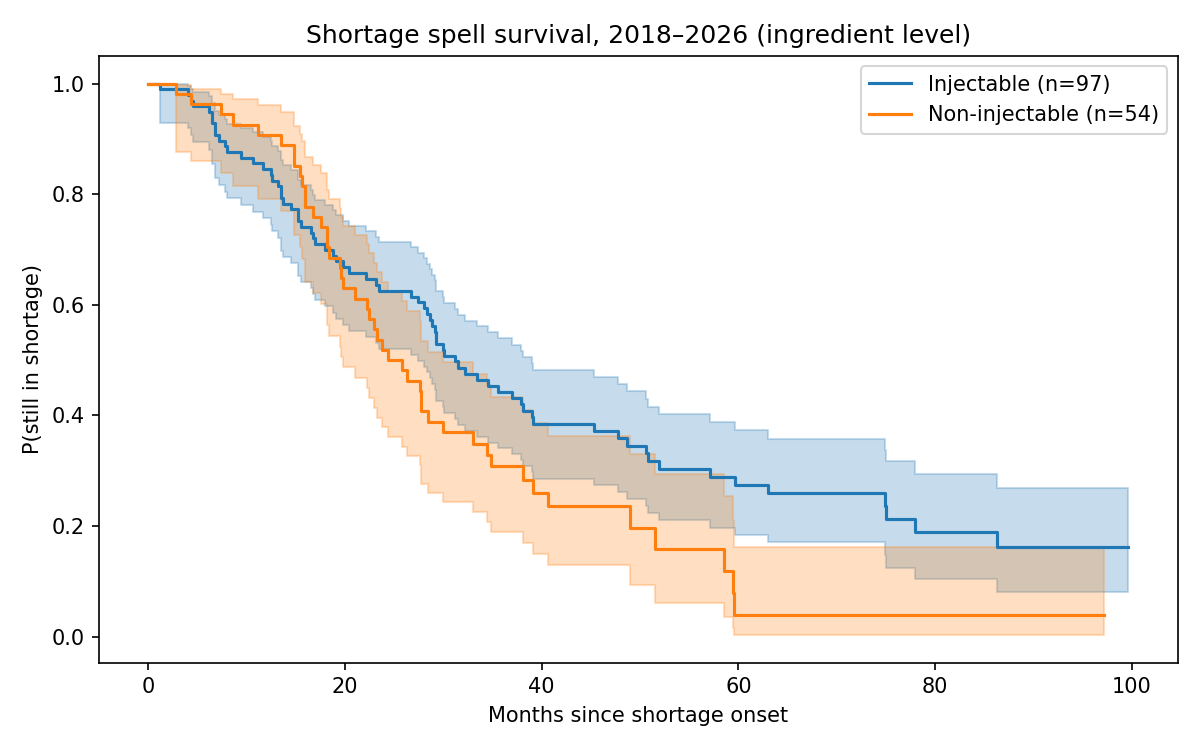
\includegraphics[width=.78\textwidth]{figures/km_injectable.png}
\caption{Kaplan--Meier survival of shortage spells, 2018--2026.}\label{fig:km}\end{figure}
\begin{figure}[H]\centering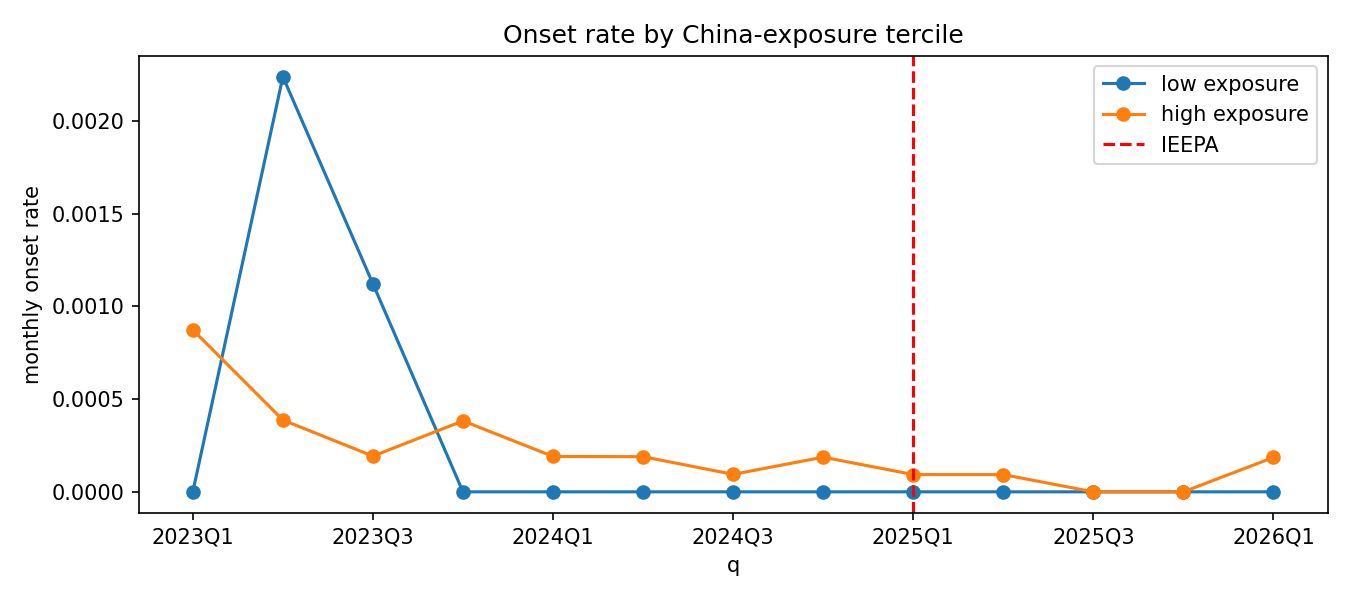
\includegraphics[width=.85\textwidth]{figures/event_study_onset.png}
\caption{Quarterly onset rates by China-exposure tercile.}\label{fig:event}\end{figure}
\begin{figure}[H]\centering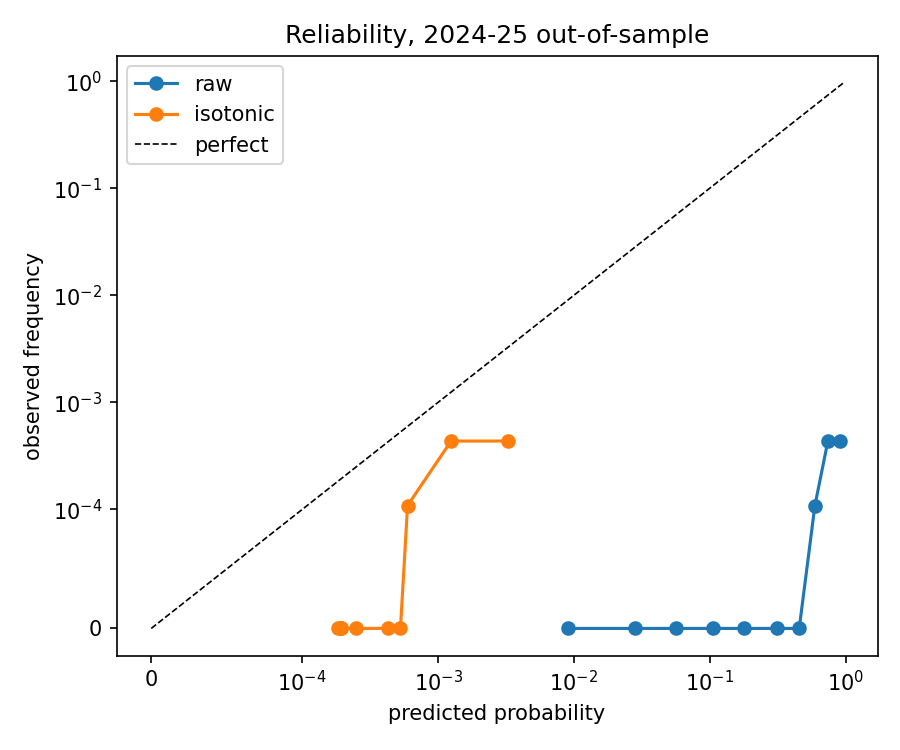
\includegraphics[width=.62\textwidth]{figures/calibration.png}
\caption{Reliability before/after isotonic recalibration (2024--25 fold).}\label{fig:calib}\end{figure}
\begin{figure}[H]\centering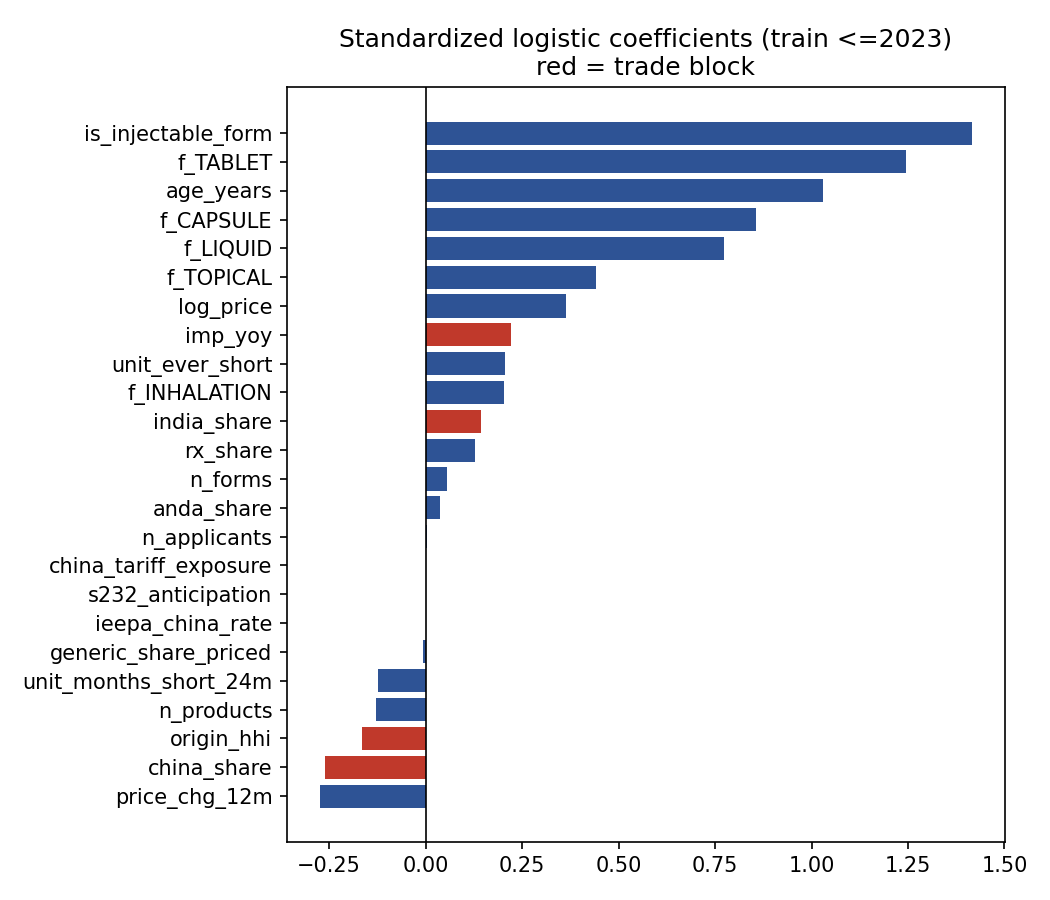
\includegraphics[width=.72\textwidth]{figures/coefficients.png}
\caption{Standardized logistic coefficients; trade block in red.}\label{fig:coef}\end{figure}

\bibliographystyle{plainnat}
\bibliography{references}
\end{document}
